\scanpage{7}
\mspage{5}
equivalently, there exists a $v\in\mathcal E^{2n-2i}$, such that the induced morphism $v:M^i-M^{2n-i}$ is an isomorphism.

One can transform this as follows:
\[
\left\{\begin{aligned}
&\exists\ v_i\in\mathcal E^{2n-2i},\quad w_i\in\mathcal E^{-(2n-2i)},\quad\text{such that one has}\\
&(w_iv_i-1)\pi_i=0,\quad(v_iw_i-1)\pi_{2n-i}=0
\end{aligned}\right.
\tag*{$(4.4)_i$}
\]
Now, without any longer supposing that $\mathcal E^*$ is realized by means of an $M^*$, one sees at once that $(4.4)_i$ implies $(3.1)_i$ and $(3.2)_i$. Indeed, replacing $v,w$ if necessary by $v\pi_i=\pi_{2n-i}v$, $w\pi_{2n-i}=\pi_iw$, one can suppose $v,w$ in $\mathcal E_i^{2n-i}$, $\mathcal E_{2n-i}^i$. If then \deleted{\unsure{u}} $u\in\mathcal E^{(0)}$ is such that $\mathcal E_i^{2n-i}u=0$, hence $vu=0$, one will have $wvu\pi_i\deleted{=0}=0$ i.e. $wv\pi_i u=0$ hence $\pi_i u=0$ (since $wv\pi_i=\pi_i$). Likewise for $(3.2)_i$, using the last relation $(4.4.)_i$.

\margin{\figure{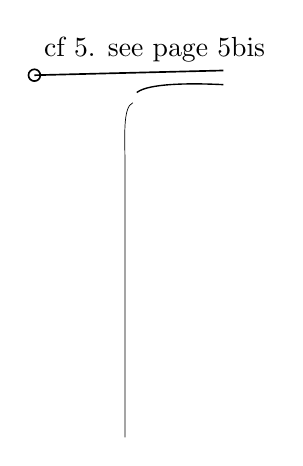
\begin{tikzpicture}[x=1cm,y=1cm]
\node[anchor=south west] at (0,4.65) {cf 5. see page 5bis};
\draw[line width=.6pt] (0,4.6)--(2.4,4.66);
\draw[line width=.6pt] (0,4.6) circle (.075);
\draw[line width=.5pt] (1.3,4.38) .. controls (1.45,4.5) and (2.0,4.5) .. (2.4,4.48);
\draw[line width=.25pt] (1.25,4.25) .. controls (1.12,4.2) and (1.15,3.8) .. (1.15,3.5)--(1.15,0);
\end{tikzpicture}}}

6. We shall study in more detail a case where the conditions $(4.4)$ are satisfied. For this, let us again start from the particular case $M^*$, \inserted{\figure{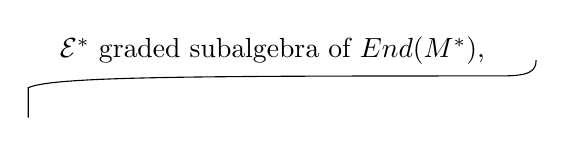
\begin{tikzpicture}[x=1cm,y=1cm]\node at (0,.35) {$\mathcal E^*$ graded subalgebra of $\operatorname{End}(M^*)$,};\draw (-3.1,-.5)--(-3.1,-.12) .. controls (-2.8,.02) and (-1.1,.03) .. (2.9,.03) .. controls (3.25,.03) and (3.35,.08) .. (3.35,.23);\end{tikzpicture}}} and suppose that we have an
\[
L\in\mathcal E^{(2)}
\tag{6.0}
\]
which has the property that
\mspage{6}
